\documentclass[border=0.8cm]{standalone}

\usepackage{tikz}
\usetikzlibrary{automata, positioning, arrows}

\tikzset{
  ->, % makes the edges directed
  >=stealth', % makes the arrow heads bold
  node distance=3cm, % specifies the minimum distance between two nodes. Change if necessary.
  every state/.style={thick, fill=gray!10}, % sets the properties for each ’state’ node
  initial text=$ $, % sets the text that appears on the start arrow
}
\begin{document}
    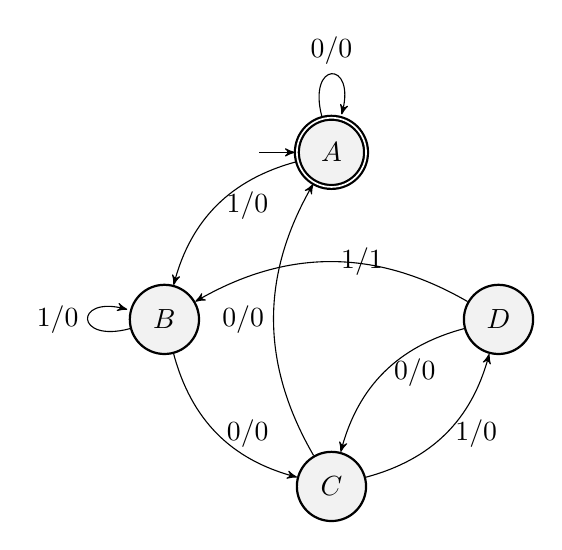
\begin{tikzpicture}
        % tikz code goes here

        \node[state, initial, accepting] (1) {$A$};
        \node[state, below left of=1] (2) {$B$};
        \node[state, below right of=2] (3) {$C$};
        \node[state, above right of=3] (4) {$D$};

        \draw (1) edge[above, bend right, right = 0.1] node{$1/0$} (2)
        (1) edge[loop above] node{$0/0$} (1)
        (2) edge[loop left] node{$1/0$} (2)
        (2) edge[below, bend right, right = 0.1] node{$0/0$} (3)
        (3) edge[left, bend left,left=0.2] node{$0/0$} (1)
        (3) edge[below, bend right, right = 0.2] node{$1/0$} (4)
        (4) edge[below, bend right, right = 0.2] node{$0/0$} (3)
        (4) edge[right, bend right, right = 0.2] node{$1/1$} (2);
        
        \end{tikzpicture}

\end{document}
